


\begin{frame}[c]{Resumo do Conteúdo Programático}
	\vspace{2mm}
	\centering
	\makebox[1\textwidth][c]{       %centering table
		\scalebox{0.95}{
			{\renewcommand{\arraystretch}{1.2}
				\fontsize{9pt}{13}\selectfont{
%	\resizebox{0.8\textwidth}{0.42\textheight}{
%		% \makebox[1\textwidth][c]{       %centering table
%		% \scalebox{0.75}{
%		{\renewcommand{\arraystretch}{1.5}
%			\fontsize{10pt}{14pt}\selectfont{
				\pgfplotstabletypeset[col sep=&,
				string type,
				column type=l,
				% columns/Nome Completo/.style={column name={Nome Completo}, column  type={l}},
				columns/0/.style={column name=N,column type={|l|}},
				columns/1/.style={column name=Aulas, column type={l}},
				columns/2/.style={column name=Mês, column type={|l}},
				columns/3/.style={column name=Data, column type={|l}},
				columns/4/.style={column name={Conteúdo Previsto}, column type={|l}},
				every head row/.style={before row=\hline,after row=\hline},
				every last row/.style={after row=\hline},
				after row={\hline},
				every head row/.style={
					before row={
						\noalign{\hrule height 1.5pt}
					},
					after row={
						\hline
					},  
				},
				every last row/.style={
					after row=\noalign{\hrule height 1.5pt}
				},
				col sep = comma,
				every head row/.style={
					before row={\hline\rowcolor{yellow!25}},after row=\hline
				},
				every row no 8/.style={
					before row={\rowcolor{red!25}}
				},
				% every row no 5/.style={
				% 	before row={\rowcolor{red!25}}
				% },
				% every row no 6/.style={
				% 	before row={\rowcolor{red!25}}
				% },
				% every row no 9/.style={
				%     before row={\rowcolor{red!25}}
				% },
				every row no 6/.style={
					before row={\rowcolor{green!25}}
				},
				every row no 13/.style={
					before row={\rowcolor{green!25}}
				},
				every row no 14/.style={
					before row={\rowcolor{green!25}}
				},
				]{\cronograma}
		}}
		% }
		 }
	}
\end{frame}



\begin{frame}[t]{Quem sou eu?}
% 	\begin{minipage}[r]{.15\textwidth}
% % 	\vspace{1cm}
%     \end{minipage}
    \hfill\begin{flushright}% or better \raggedleft see comments below
  \vspace{-2em}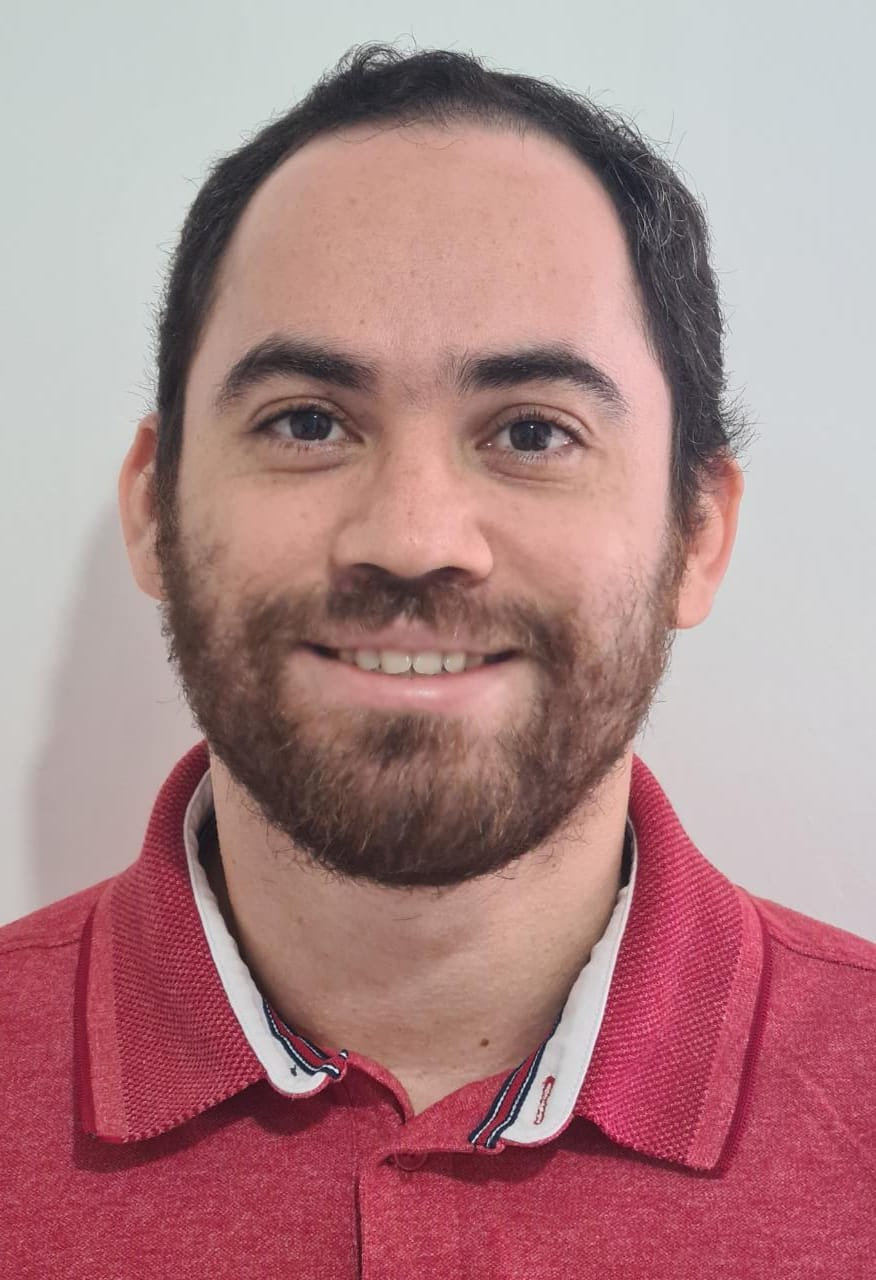
\includegraphics[scale=0.09]{imagens/fig-s20-plus-foto-lattes.jpeg}
 \end{flushright}

    \vspace{-9em}
    
    \begin{minipage}{.7\textwidth}
      \fontsize{10pt}{12}\selectfont{
    	\begin{itemize}%[<+->]  
    	    \item \autor, 39 anos (12/02)
    	    \item Sou técnico em Análise e Desenvolvimento de Sistema. Possuo Bacharelado nos cursos de Ciência da Computação (2011) e Sistemas de Informação (2016), participei do programa de Residência em Engenharia e Reuso de Software por meio da parceria da RiSE, Porto Digital e CPNq (2012). Tenho mestre e doutor em Ciência da Computação pelo CIn/UFPE. Atuo na indústria com desenvolvimento de software e na academia como professor.
        	\begin{itemize}%[<+->]  
        	    \item Java, Kafka, Postgresql, Docker, Angular, Spring...
        	    \item Análise e Desenvolvimento de Sistemas, Sistemas de Informação, Redes de Computadores.
        	\end{itemize}
    	\end{itemize}
    	}\par
    \end{minipage}

	\vspace{1em}
	\centering
\fontsize{20pt}{15.2}\selectfont{
    \url{http://www.brunomaciel.com}
	\vspace{1em}
	}\par
	
	
\end{frame}


\begin{frame}{Quem sou eu?}
% 	\begin{minipage}[r]{.15\textwidth}
% % 	\vspace{1cm}
%     \end{minipage}
%     \hfill\begin{flushright}% or better \raggedleft see comments below
%   \vspace{-3em}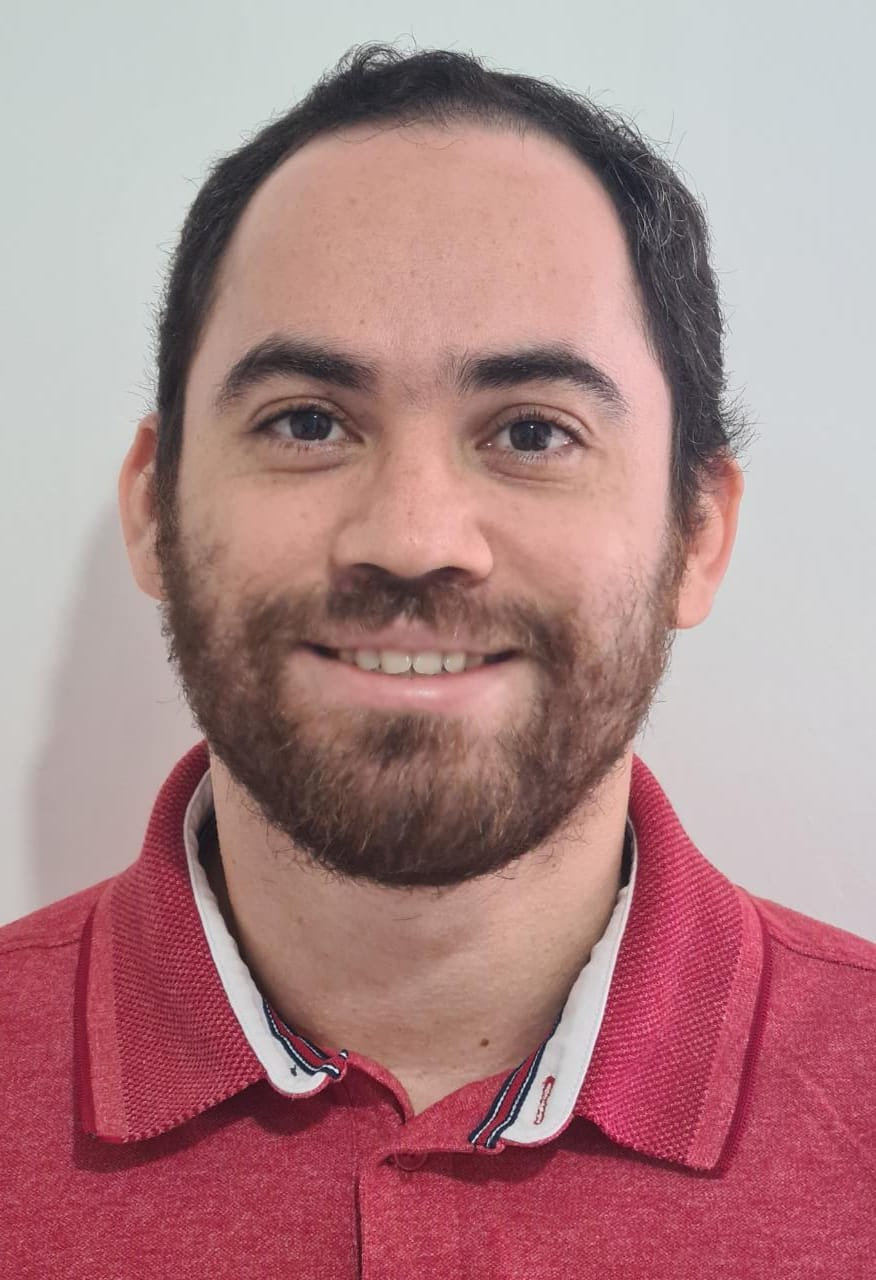
\includegraphics[scale=0.09]{imagens/fig-s20-plus-foto-lattes.jpeg}
%  \end{flushright}

%     \vspace{-10em}
    
    \begin{minipage}{.8\textwidth}
      \fontsize{10pt}{12}\selectfont{
    	\begin{itemize}%[<+->]  
    	   % \item \autor, 39 anos (12/02)
    	    \item Técnico em Análise e Desenvolvimento de Software, 2019-2020
    	    \item Doutor em Ciência da Computação, 2015-2020
    	    \item Mestre em Ciência da Computação, 2012-2014
    	    \item Especialista em Engenharia e Reúso de Software, 2011-2012
    	    \item Graduado em Sistemas de Informação, 2016-2016
    	    \item Graduado em Ciência da Computação, 2007-2011
    	    \item Técnico em Análise e Desenvolvimento de Software, 2007-2007
    	    \item CV completo \url{http://bit.ly/brunomaciel-lattes}
    	\end{itemize}
    	}\par
    \end{minipage}

	\vspace{1em}
	\centering
\fontsize{20pt}{15.2}\selectfont{
E-mail:	facir@brunomaciel.com
	\vspace{1em}
	}\par
	
\end{frame}


\begin{frame}{}
    \fontsize{14pt}{15.2}\selectfont{
	Apresentação pessoal, integração com a turma, introdução de conceitos básicos de banco de dados e despertar curiosidade alunos sobre o tema.
	
	\vspace{1em}
	}\par
	\vspace{1em}
\end{frame}


\begin{frame}{Aplicação de Avaliação}
    \fontsize{14pt}{15.2}\selectfont{
	Datas importantes
	\vspace{1em}
	}\par
	
	\fontsize{12pt}{15}\selectfont{
	\begin{itemize}%[<+->]  
	   % \item 30/09/2020 - Simulado da Primeira Avaliação (1A)
	    \item \textbf{01/04/2022 - Primeira Avaliação NP1}
	    \item 15/04/2022 - Feriado
	   % \item \textbf{18/11/2020 - Defesa dos projetos}
	   % \item 03/06/2020 - Simulado da Segunda Avaliação (2A)
	   % \item \textbf{01/04/2020 - Avaliação}
	    \item \textbf{20/05/2022 - Segunda Avaliação NP2} 
	    \item \textbf{03/06/2022 - Substitutiva}
	\end{itemize}
	
	}\par
	
	\vspace{1em}
\end{frame}



\begin{frame}{Compromisso semanal}
%     \fontsize{14pt}{15.2}\selectfont{
% 	Datas importantes
% 	\vspace{1em}
% 	}\par
	
	\fontsize{12pt}{15}\selectfont{
	\begin{itemize}%[<+->]  
	    \item Encontros: sextas
	    \item Período: %06/02/2020 à 04/06/2020
	    \item Início: 19h
	    \item Térmico: 21h50m
	   % \item Intervalo: 20h10m até 20h20m (a discutir)
	    \item Sala: 33
	\end{itemize}
	
	}\par
	
	\vspace{1em}
\end{frame}


\begin{frame}{Metodologia das Aulas}
Aulas:

    \fontsize{10pt}{12}\selectfont{
    \begin{itemize}%[<+->]  
        \item 19h-20h
        \item 20h-20h20m (intervalo)
        \item 20h20m-21h50m
	\end{itemize}
	}\par
	\vspace{0.5em}
	\fontsize{12pt}{15}\selectfont{
		\begin{itemize}%[<+->]  
	    \item Resolução de dúvidas gerais: 19h até 19h30m (30min)
	   % \item Revisão da aula passada: 19h20m até 19h40m (20min)
	   % \item Exercício em sala de aula: 19h40m até 19h50m (10min)
	    \item Adição de novos conteúdos: 19h30m até 21h50m
	   % \item Revisão/dúvidas do novo conteúdo: 21h20m até 21h30m (10m)
	\end{itemize}
	}\par
	\vspace{1em}
\end{frame}

\begin{frame}{Metodologia das Avaliação}

	\fontsize{12pt}{15}\selectfont{
	\begin{itemize}%[<+->]  
	    \item Primeira nota: %(exercício + prova)
	        \begin{itemize}%[<+->]  
%        	    \item Exercícios (peso +1)
        	    \item Prova escrita (peso 10)
        	\end{itemize}
    	\item Segunda nota: %(exercício + prova + projeto)
	        \begin{itemize}%[<+->]  
        	   % \item Exercícios (peso 1,5)        	    
        	   % \item Projeto (peso 1,5)
        	   % \item Participação - Frequência em aulas (peso 1)
        	    \item Prova escrita (peso 10)
        	\end{itemize}
	\end{itemize}
	}\par
	\vspace{1em}
\end{frame}

% \begin{frame}{Avisos}

% 	\fontsize{12pt}{15}\selectfont{
% 	\begin{itemize}%[<+->]  
% 	    \item Frequência escolar:
% 	        \begin{itemize}%[<+->]  
%         	    \item Número de faltas maior que 25\% = |Reprovado por faltas|
%         	    \item Cada dia de aula faltado equivale à 3 faltas;
%         	    \item Há 15 dias de aulas no cronograma |15 = 100\%|;
%         	    \item 4 dias faltados equivale a $\pm$ 26\%.
%          	\end{itemize}
%     	\item Atraso na entrega de atividade:
% 	        \begin{itemize}%[<+->]  
%         	    \item Cada dia atrasado tem penalidade de menos 10\% do peso.
%         	    \item Tempo máximo de atraso tolerado = 7 dias.
%         	\end{itemize}
% 	\end{itemize}
% 	}\par
% 	\vspace{1em}
% \end{frame}



\begin{frame}[t]{Ementa}
\vspace{1cm}
	\fontsize{12pt}{16}\selectfont{
	Conceituação de Organização e Arquitetura de Computadores e Máquinas Multiníveis. Organização de Sistemas Computacionais: CPU, Memória, Entradas e Multimídia e Barramentos. Nível Lógico Digital: Unidade Lógica e Aritmética, Organização de Memória, Clock e Registradores. Nível de Microarquitetura: Fluxos de Dados, Temporização do Fluxo de Dados, Operação de Memória, Microinstruções, O Mic-1, Exemplo de Macroarquitetura e Projeto do Nível de Microarquitetura (forma introdutória).
	}\par
	\vspace{1em}
\end{frame}

\begin{frame}[t]{Objetivos Gerais}
\vspace{1cm}
	\fontsize{12pt}{16}\selectfont{
	Entender o hardware de um sistema computacional. Entender o funcionamento dos vários módulos que compõem um sistema computacional.Conhecer a organização interna dos computadores, para análise da otimização do uso de seus componentes em aplicações das áreas de informação, comunicação e processos de controle.
	}\par
	\vspace{1em}
\end{frame}

\begin{frame}{Competências Específicas}

	\fontsize{12pt}{15}\selectfont{
% 	\begin{itemize}%[<+->]  
	   % \item 
	    Compreender a estrutura fundamental dos computadores e sua consequente organização, entendendo sua evolução, os conceitos fundamentais de seu próprio funcionamento e de seus componentes elementares, como processadores, memórias, sistemas de comunicação e dispositivos de entrada/saída.
% 	\end{itemize}
	}\par
	\vspace{1em}
\end{frame}



\begin{frame}{Avaliação}

	\fontsize{12pt}{15}\selectfont{
    Serão feitas avaliações, assim distribuídas:\vspace{1em}
	    
	\begin{itemize}%[<+->]  
	    \item Duas Notas do Professor (NP) para as atividades curriculares, com peso 4 (quatro) cada uma, na composição da nota semestral de cada disciplina;
	    
        \item Uma nota referente ao Projeto Integrado Multidiscipinar (PIM), com peso 2 (dois) no cálculo da Média Semestral (MS) de cada disciplina. Esse Projeto será desenvolvido durante o semestre.
        
        \item A MS será: (NP1 x 4 + PIM x 2 + NP2 x 4) / 10. Para a aprovação, a MS deverá ser igual ou superior a 5,0; é exigida a frequência mínima de 75\%. 
        
        \item O desempenho do aluno é avaliado numa escala de 0 (zero) a 10 (dez).
	\end{itemize}
	}\par
	\vspace{1em}
\end{frame}



\begin{frame}[t]{Bibliografia básica}
    \fontsize{12pt}{15.2}\selectfont{
	\vspace{1em}
	    \begin{itemize}
            \item DELGADO, José; RIBEIRO, Carlos. Arquitetura de Computadores. São Paulo: LTC, 2017.
            
            \item STALLINGS, W. Arquitetura e organização de computadores.10. ed. São Paulo: Prentice Hall, 2017.
            
            \item WIDMER, Neal S; TOCCI, Ronald J; MOSS, Gregory L. Sistemas Digitais. 12 ed. São Paulo: Pearson Education do Brasil, 2018.
            
            \item Mais informações é possível encontrar na ementa.
	    \end{itemize}
	}\par
\end{frame}


% \begin{frame}{Google sala de aula}
	
%     \hfill\begin{flushright}% or better \raggedleft see comments below
% 	 \vspace{-10mm}\includegraphics[width=25mm]{imagens/fig-qrcode-classroom.png}
% 	\end{flushright}


% %    \begin{wrapfigure}{r}{30mm}
% %    \vspace{-15mm}\qrcode[height=1in]{https://classroom.google.com}
% % 	\includegraphics[keepaspectratio=true,scale=0.4,trim=0cm 0 0 5cm]{imagens/qrcode.png}
% %	\end{wrapfigure}
% 	\vspace{-15mm}
	
%     \fontsize{14pt}{15.2}\selectfont{
% 	\vspace{1em}Código da turma \fontsize{34pt}{15.2}\selectfont{vigm76e}
% 	}\par
% 	\vspace{0.5em}

% 	\fontsize{10pt}{12}\selectfont{
% 	Vamos ter como recurso complementar o Google Sala de Aula [classroom]. Por lá vou deixar o material (slides, referências, atividades, etc.) que vocês vão utilizar durante o curso. Não preocupem-se, também vou deixar uma cópia do material (slides e atividades) disponível em pendrive e levarei comigo durante as aulas para os alunos que não puderem acessar o Google Classroom.
% 	\vspace{1em}
	
	
	
% 	Como usar o google sala de aula?

%     Use este tutorial \url{https://www.youtube.com/watch?v=l4oSdhLS5fQ} [vídeo] para te ajudar a entender o Google Classroom.

%     Clique na \url{https://classroom.google.com} para entrar no Google Classroom.

% 	}\par
% \end{frame}



